\documentclass{beamer}

% to include graphics
\usepackage{graphicx}

% to include hyperlinks
\usepackage{hyperref}

% divide slides into columns
\usepackage{multicol}


\usetheme{Copenhagen}
\usecolortheme{beaver}

\usepackage{graphicx}
\usepackage{subcaption}

\title{Cluster Progress}
\date{\today}

\begin{document}

%----------BEGIN TITLE----------

\begin{frame}
  \maketitle
\end{frame}

%-----------END TITLE-----------

%----------BEGIN NAS-1----------

\begin{frame}
  \frametitle{NAS-1 Emergency Mode}

  \begin{itemize}    
  \item NAS-1 booted into emergency mode after being turned off for the Hurricane.
  \item An error message appeared, saying that there was an, ``Un-Correctable DRAM ECC Error at CPU02/DIMM2A''
    %only after a couple of reboots though. Turn on = emercency mode, reboot, emergency mode, reboot emergency mode, left for the weekend,
    %turn off to mess with the APC, turn on, bam. 
  \item Michael and I swapped the RAM in slots 2A and 3A to make sure the issue was with the RAM instead of with the slot. 
  \item However, upon rebooting the error message did not appear, and NAS-1 booted into emergency mode again.
    %trying to turn it all the way off now
  \end{itemize}

  \begin{figure}[H]
    \begin{center}
      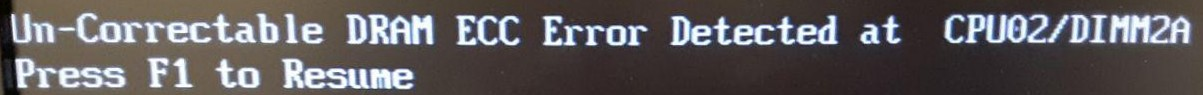
\includegraphics[width=0.5\textwidth]{DRAM_error.jpg}
    \end{center}
  \end{figure}

  \begin{figure}[H]
    \begin{center}
      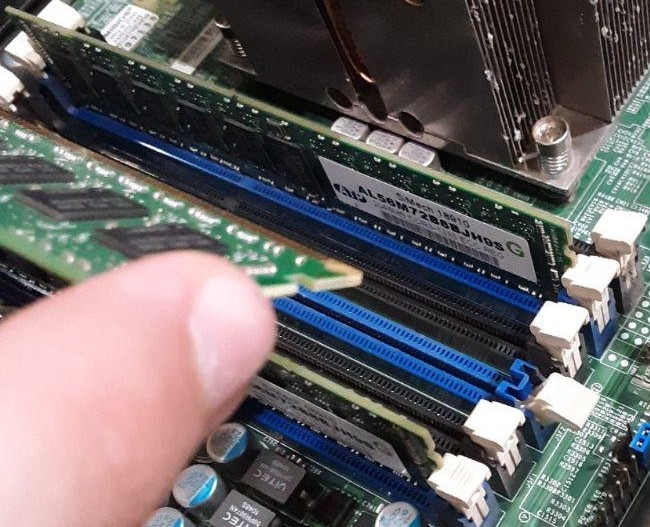
\includegraphics[width=0.5\textwidth]{RAM.jpg}
    \end{center}
  \end{figure}
  

\end{frame}
%-----------END NAS-1-----------

%t3 cluster meetings: need to get access to lxplus to sign up, and CERN lightweight acct doesnt have accest to lxplus.
% solution: contact  former secretariat and renew my affiliation

%OSG: provided me a link to the guide on how to renew host certs, but no word back yet on my account status. 

\end{document}
